\problemname{The Abacus}

\begin{figure}[h] 
\begin{center}
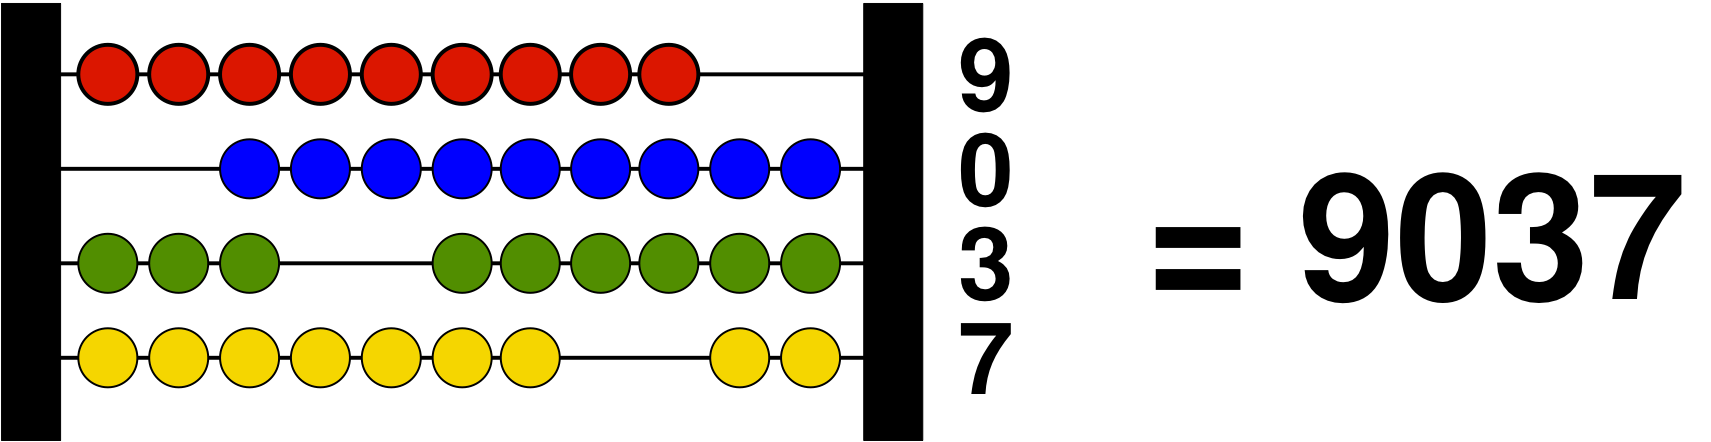
\includegraphics[width=10cm]{kulram0.png}
\caption{This is what Simon's abacus (with $R=4$) could have looked like before he
  started eating the beads. Back then it was easy to translate the position into a decimal number.}
\end{center} 
\end{figure}
\vspace{-2cm}

Little Simon has received an abacus as a present. The abacus has $R$ rows and
each row originally had 9 beads, so that one could represent
$R$-digit decimal numbers -- one digit per row. If a row had $X$
beads on the left side, then a gap, and the remaining beads on the right side, the row represented the digit X.

Unfortunately, Simon thought the beads on the abacus looked very tasty, and simply ate some of them. However, there is at least one bead left on each row.

Simon quickly learned to count on his new abacus. He represents
the number where all beads are on the right side as the number 0, and then adds 1
just as he would have done on a regular abacus, by moving one
bead from right to left on the lowest row that has any bead
remaining on the right side (let us call it the {\em shifting row}) and
moving all beads on the rows below the shifting row to the right side
(unless the shifting row is the bottom row). If 1 is added when the
beads on {\em all} rows are already on the left side (so that there is no shifting row) the result becomes 0.

\begin{figure}[h] 
\begin{center}
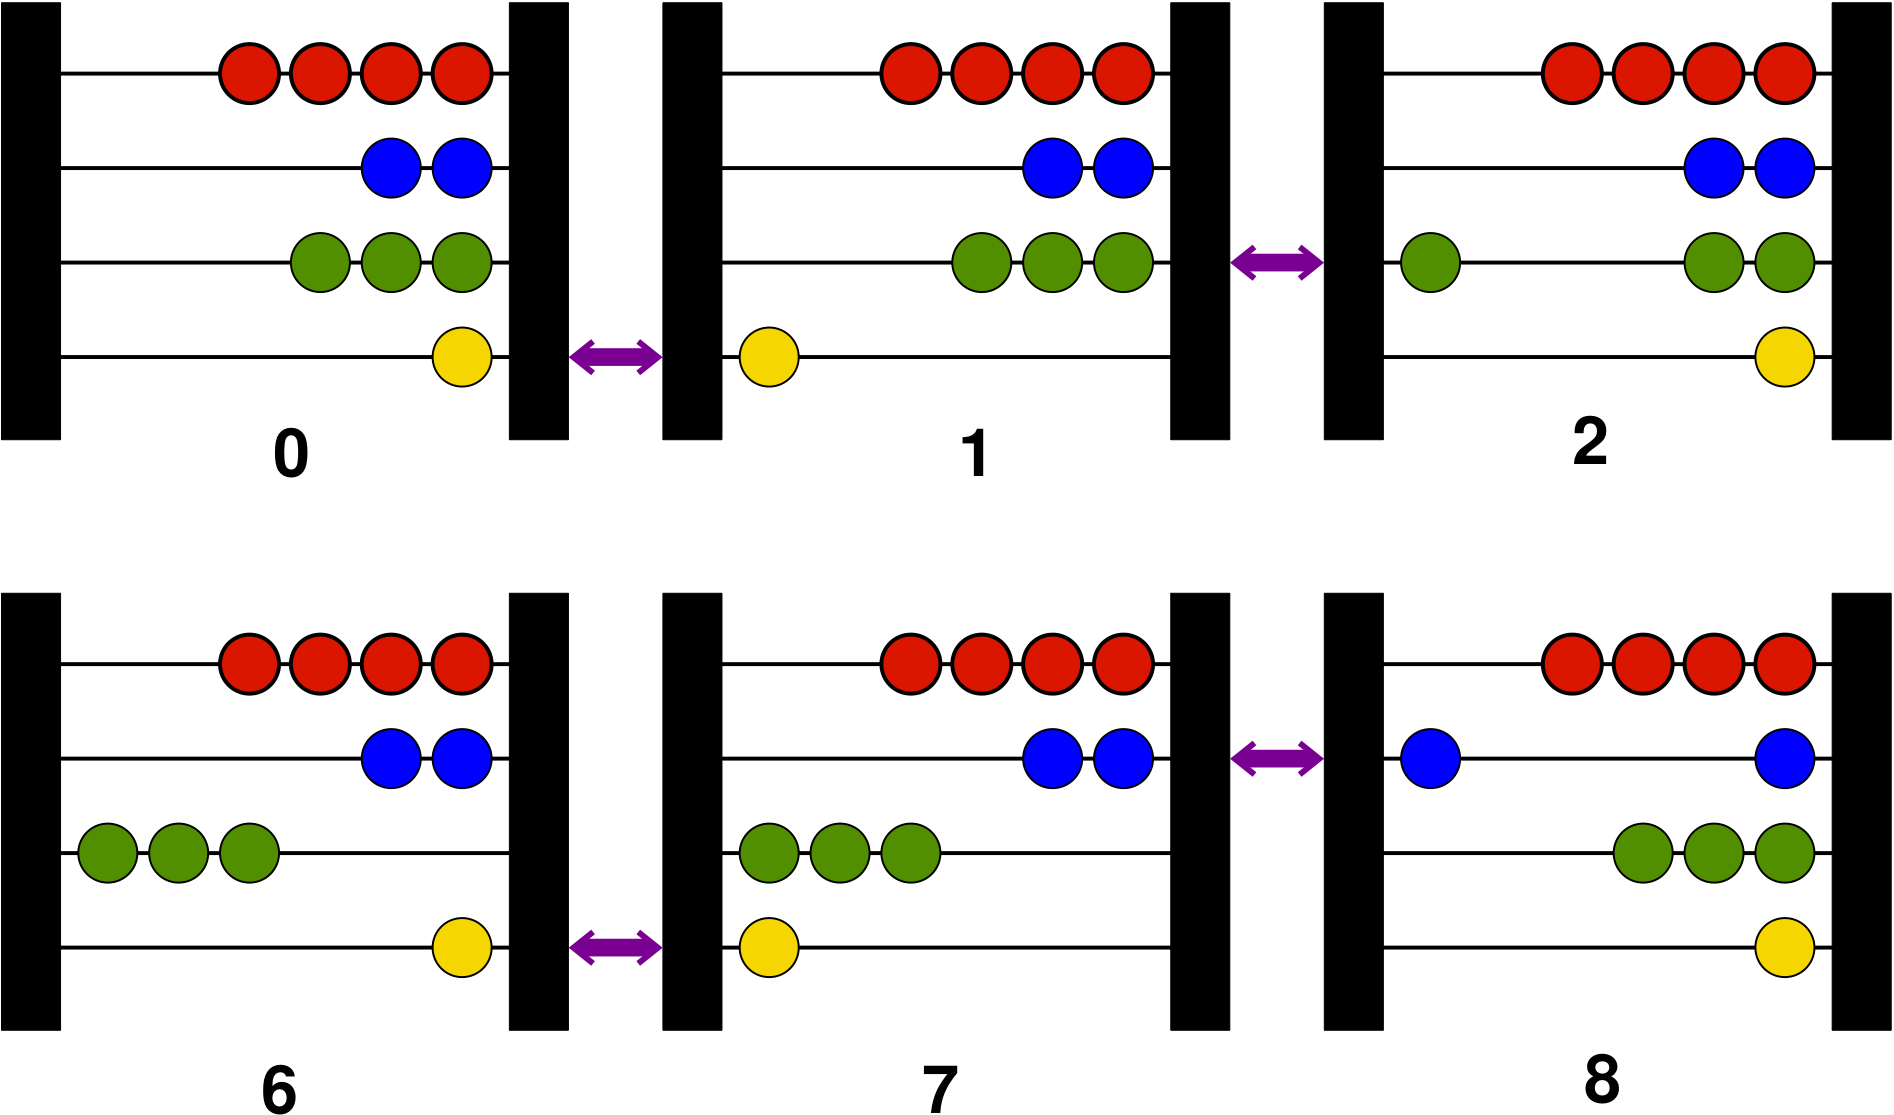
\includegraphics[width=8cm]{kulram.png}
\caption{Some examples of how Simon adds 1 on the abacus found in the first two samples. The double arrow
  marks the ``shifting row'' in the different additions.}
\end{center} 
\end{figure}

Simon is counting the grains of sand in his sandbox and would need help
writing a program that, given a certain initial position on the abacus,
computes what the abacus looks like after he has added
1 a total of $N$ times.

\section*{Input}
The first line contains the number of rows $R$. Then follow $R$ lines with two integers each, the number of beads
on the left and right side of each row (from top to bottom). Finally there is a line with
the positive integer $N$. 

\section*{Output} 

The program should output $R$ lines with two numbers on
each line: the number of beads on the left and right side of each row
after the additions.

\section*{Scoring}

For test cases worth 20 points, $R=4$, $N\le 100$, and there are 2 beads
on each row.\\
For test cases worth an additional 40 points, $R=4$ and $N\le 10{,}000$.\\
For test cases worth 40 points, $R\le 12$ and $N\le 10^{12}$.
